\chapter{Лабораторная работа 5 \\
Проектирование автогенератора на основе обратной связи}

Цель работы: изучить основы моделирования автогенераторов в среде Advanced Design System, научиться проектировать и выполнять моделирование автогенератора.

\section{Техническое задание}

Спроектировать автогенератор на транзисторе HBFP0420.
В качестве рабочей точки принять $V_{CE} = 2~\text{В}$, $I_C = 20~\text{мА}$.
Центральная частота $RF = 1.5~\text{ГГц}$.

\section{Выполнение работы}

\subsection{Расчёт цепи смещения транзистора}

Для расчёта цепи смещения транзистора воспользуемся умным компонентом \elementname{DA\_DJTBias} из палитры \elementname{Transistor Bias}.
Соберём схему, подключив все порты транзистора и питания к соответствующим портам умного компонента (Рис.~\ref{fig:feedback_oscillator_schematic_1}).

\begin{figure}[!ht]
    \centering
    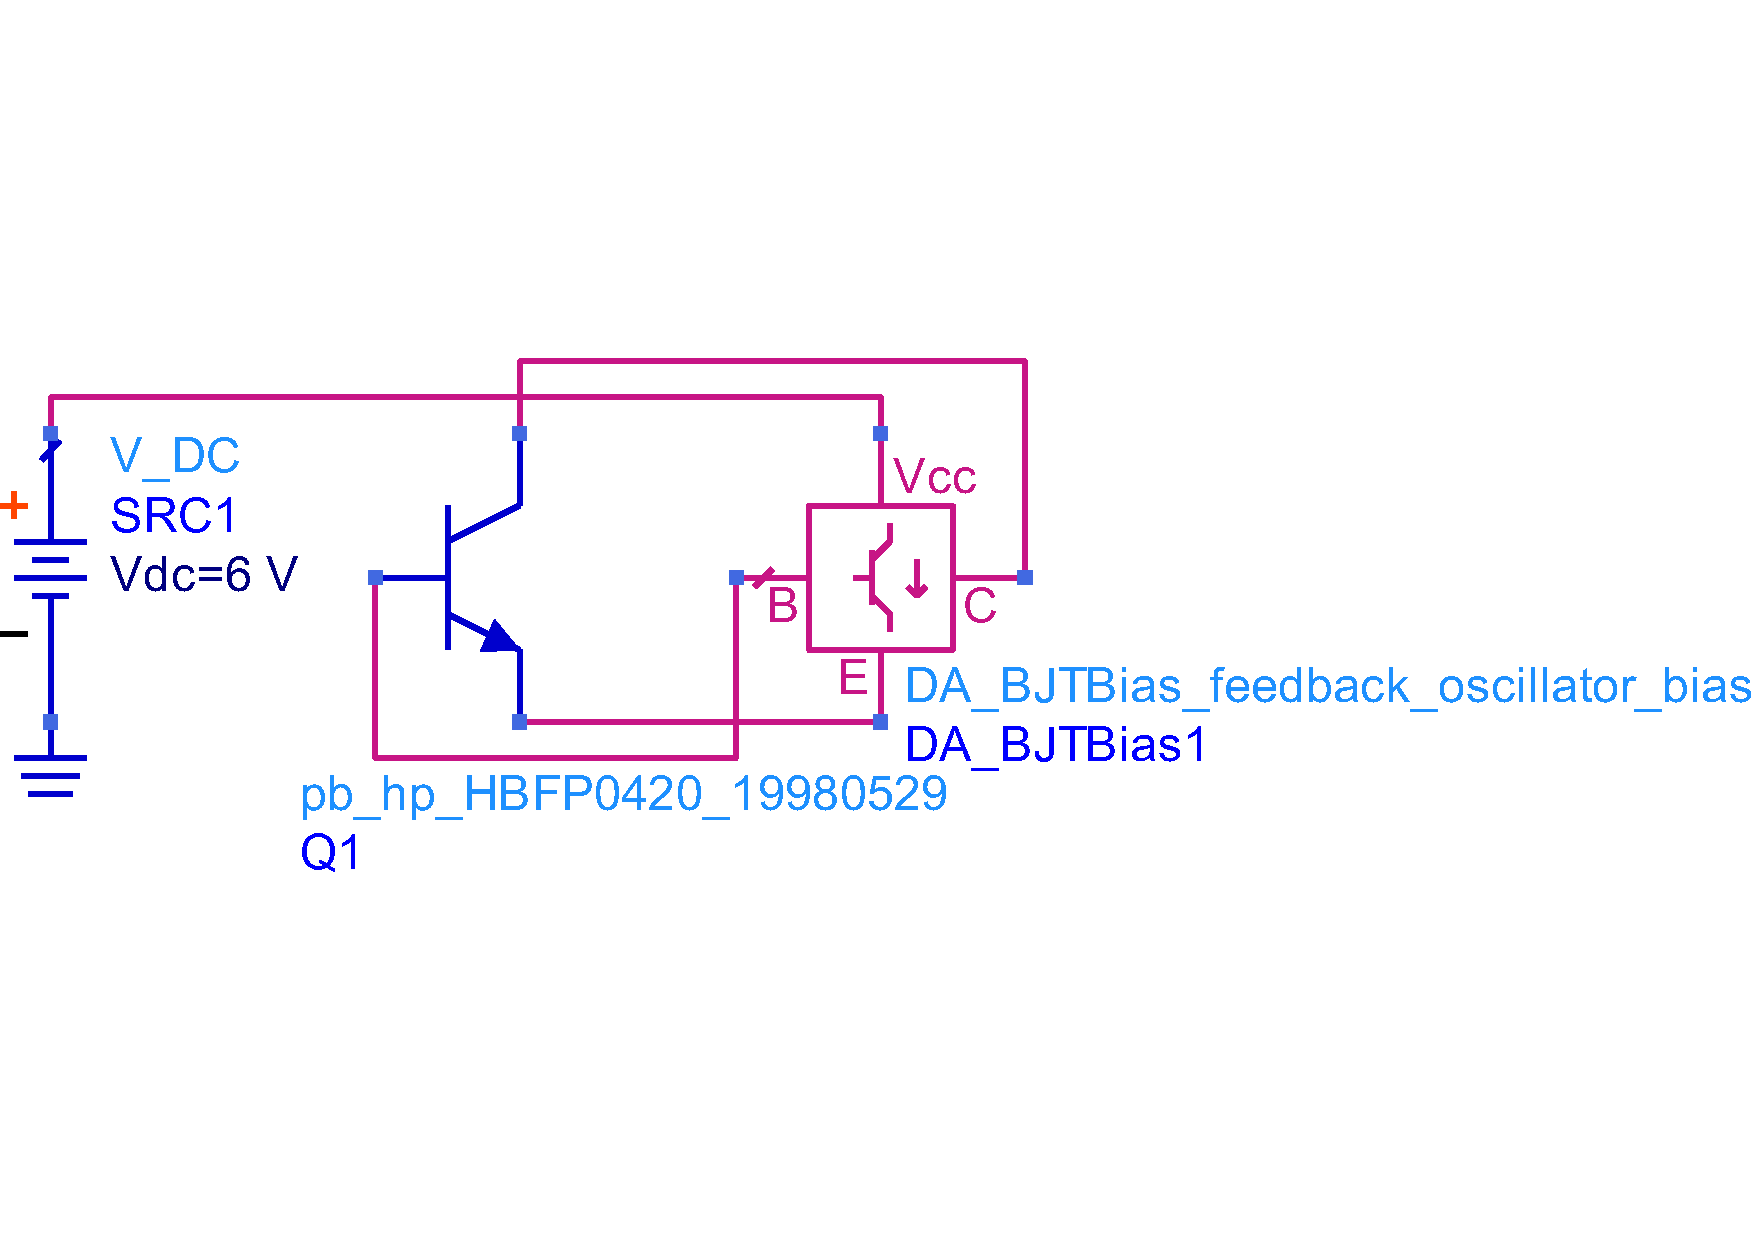
\includegraphics[width=0.9\textwidth]{feedback_oscillator_schematic_1.pdf}
    \caption{Схема расчёта цепи смещения транзистора}%
    \label{fig:feedback_oscillator_schematic_1}
\end{figure}


